%%%%%%%%%%%%%%%%%%%%%%%%%%%%%%%%%%%%%%%%%%%%%%%%%%%%%%%%%%%%%%%%%%%%%%%%%%%%%%%%%%%
%% This project aims to create the template for presentation.                   %%
%% author: Luigi Durso                                                          %%
%% contacts:                                                                    %%
%%    e-mail: luigi.durso@si2001.it                                             %%
%%    linktree: https://linktr.ee/maumneto                                      %%
%%%%%%%%%%%%%%%%%%%%%%%%%%%%%%%%%%%%%%%%%%%%%%%%%%%%%%%%%%%%%%%%%%%%%%%%%%%%%%%%%%%
\documentclass{../libs/presentation_format}
% Inserting the preamble file with the packages
%%%%%%%%%%%%%%%%%%%%%%%%%%%%%%%%%%%%%%%%%%%%%%%%%%%%%%%%%%%%%%%%%%%%%
%% This file contains the packages that can be used in the beamer. %%
%%%%%%%%%%%%%%%%%%%%%%%%%%%%%%%%%%%%%%%%%%%%%%%%%%%%%%%%%%%%%%%%%%%%%
% Package to fonts family
\usepackage[T1]{fontenc}
% Package to accentuation
\usepackage[utf8]{inputenc}
% Package to Italian language
\usepackage[italian]{babel}
% Package to Figures
\usepackage{graphicx}
\usepackage{caption}
\usepackage{subcaption}
% Package to the colors
\usepackage{color}
% Package to the colors
\usepackage{xcolor}
% Packages to math symbols and expressions
\usepackage{amsfonts, amssymb, amsmath}
% Package to multiple lines and columns in table
\usepackage{multirow, array} 
% Package to create pseudo-code
% For more detail of this package: http://linorg.usp.br/CTAN/macros/latex/contrib/algorithm2e/doc/algorithm2e.pdf
\usepackage{algorithm2e}
% Package to insert code
\usepackage{listings} 
\usepackage{keyval}
% Package to justify text
\usepackage[document]{ragged2e}
% Package to manage the bibliography
\usepackage[backend=biber, style=numeric, sorting=none]{biblatex}
% Package to facilities quotations
\usepackage{csquotes}
% Package to use multicols
\usepackage{multicol}
% Inserting the references file
\bibliography{../references.bib}

% Title
\title[Flutter-Dart]{\huge\textbf{Flutter e Dart - Le basi}}
% Subtitle
\subtitle{Flutter - Animazioni ed interazione con il dispositivo}
% Author of the presentation
\author{Luigi Durso}
% Company's Name
\institute[SI2001]{
    % email for contact
    \normalsize{\email{luigi.durso@si2001.it}}
    \newline
    \centering
    
\includegraphics[scale=0.3]{../libs/emblem.png}
    \newline
    % company name
    \company
}
% date of the presentation
\date{\today}


%%%%%%%%%%%%%%%%%%%%%%%%%%%%%%%%%%%%%%%%%%%%%%%%%%%%%%%%%%%%%%%%%%%%%%%%%%%%%%%%%%
%% Start Document of the Presentation                                           %%               
%%%%%%%%%%%%%%%%%%%%%%%%%%%%%%%%%%%%%%%%%%%%%%%%%%%%%%%%%%%%%%%%%%%%%%%%%%%%%%%%%%
\begin{document}
% insert the code style
%%%%%%%%%%%%%%%%%%%%%%%%%%%%%%%%%%%%%%%%%%%%%%%%%%%%%%%%%%%%%%%%%%%%%%%%%%%%%%%%%%%
%% This file contains the style of the codes show in slides.                     %%
%% The package used is listings, but it possible to used others.                 %%
%%%%%%%%%%%%%%%%%%%%%%%%%%%%%%%%%%%%%%%%%%%%%%%%%%%%%%%%%%%%%%%%%%%%%%%%%%%%%%%%%%%

% color used in the code style
\definecolor{codegreen}{rgb}{0,0.6,0}
\definecolor{codegray}{rgb}{0.5,0.5,0.5}
\definecolor{codepurple}{rgb}{0.58,0,0.82}
\definecolor{codebackground}{rgb}{0.95,0.95,0.92}

% style of the code!
\lstdefinestyle{codestyle}{
    backgroundcolor=\color{codebackground},   
    commentstyle=\color{codegreen},
    keywordstyle=\color{magenta},
    numberstyle=\tiny\color{codegray},
    stringstyle=\color{codepurple},
    basicstyle=\ttfamily\footnotesize,
    frame=single,
    breakatwhitespace=false,         
    breaklines=true,                 
    captionpos=b,                    
    keepspaces=true,                 
    numbers=left,                    
    numbersep=5pt,                  
    showspaces=false,                
    showstringspaces=false,
    showtabs=false,                  
    tabsize=2,
    title=\lstname 
}

\lstset{style=codestyle}

\lstset{basicstyle=\ttfamily,
	showstringspaces=false,
	commentstyle=\color{red},
	keywordstyle=\color{blue},
	inputencoding=utf8,
	extendedchars=true
}


%% ---------------------------------------------------------------------------
% First frame (with tile, subtitle, ...)
\begin{frame}{}
    \maketitle
\end{frame}

%% ---------------------------------------------------------------------------
% Table of content frame
\begin{frame}{Sommario}
    \begin{multicols}{2}
        \tableofcontents
    \end{multicols}
\end{frame}

%% ---------------------------------------------------------------------------

\section{Lezione precedente}
\begin{frame}{Un po' di codice}
	\begin{tabular}{lll}
		\raisebox{-.5\height}{
\includegraphics[scale=0.3]{../libs/Developer-Friendly.png}}
		\emph{Analizziamo l'elaborato precedente!}\\
	\end{tabular}
\end{frame}

%% ---------------------------------------------------------------------------

\section{Animazioni}
\begin{frame}{Gestire le animazioni}
	\emph{Come possiamo animare la nostra app:}
	\begin{itemize}
		\item Gestire manualmente le anumazioni con gli animation controller;
		\item Creare dei  widget che estendano \emph{Animated­Widget};
		\item Possiamo gestire l'animazione con un \emph{AnimatedBuilder};
		\item Più semplicemente, usiamo packages di widget animati oppure widget built-in animati (Es. AnimatedContainer) \href{https://docs.flutter.dev/development/ui/widgets/animation}{\beamergotobutton{Catalogo}}
	\end{itemize}
	\centering
	\href{https://docs.flutter.dev/development/ui/animations/tutorial}{\beamergotobutton{Documentazione}}
\end{frame}

%% ---------------------------------------------------------------------------

\section{Funzionalità del dispositivo}
\begin{frame}{Funzionalità del dispositivo}
	\emph{Come possiamo sfruttare il nostro dispositivo}
	\begin{itemize}
		\item Abbiamo già visto come persistere i dati con gli \emph{Hydrated BLoC};
		\item Possiamo recuparare immagini dal filesystem o dalla fotocamera \href{https://pub.dev/packages/image_picker}{\beamergotobutton{Package}}
		\item Gestire informazioni sulla nostra posizione \href{https://pub.dev/packages/location}{\beamergotobutton{Package}}
	\end{itemize}
\end{frame}

%% ---------------------------------------------------------------------------

\section{Esercitazione}
\begin{frame}{Migliorare la precedente esercitazione}
	\begin{minipage}[0.2\textheight]{\textwidth}
		\begin{columns}[T]
			\begin{column}{0.4\textwidth}
				\begin{figure}[htpb]
					\centering
					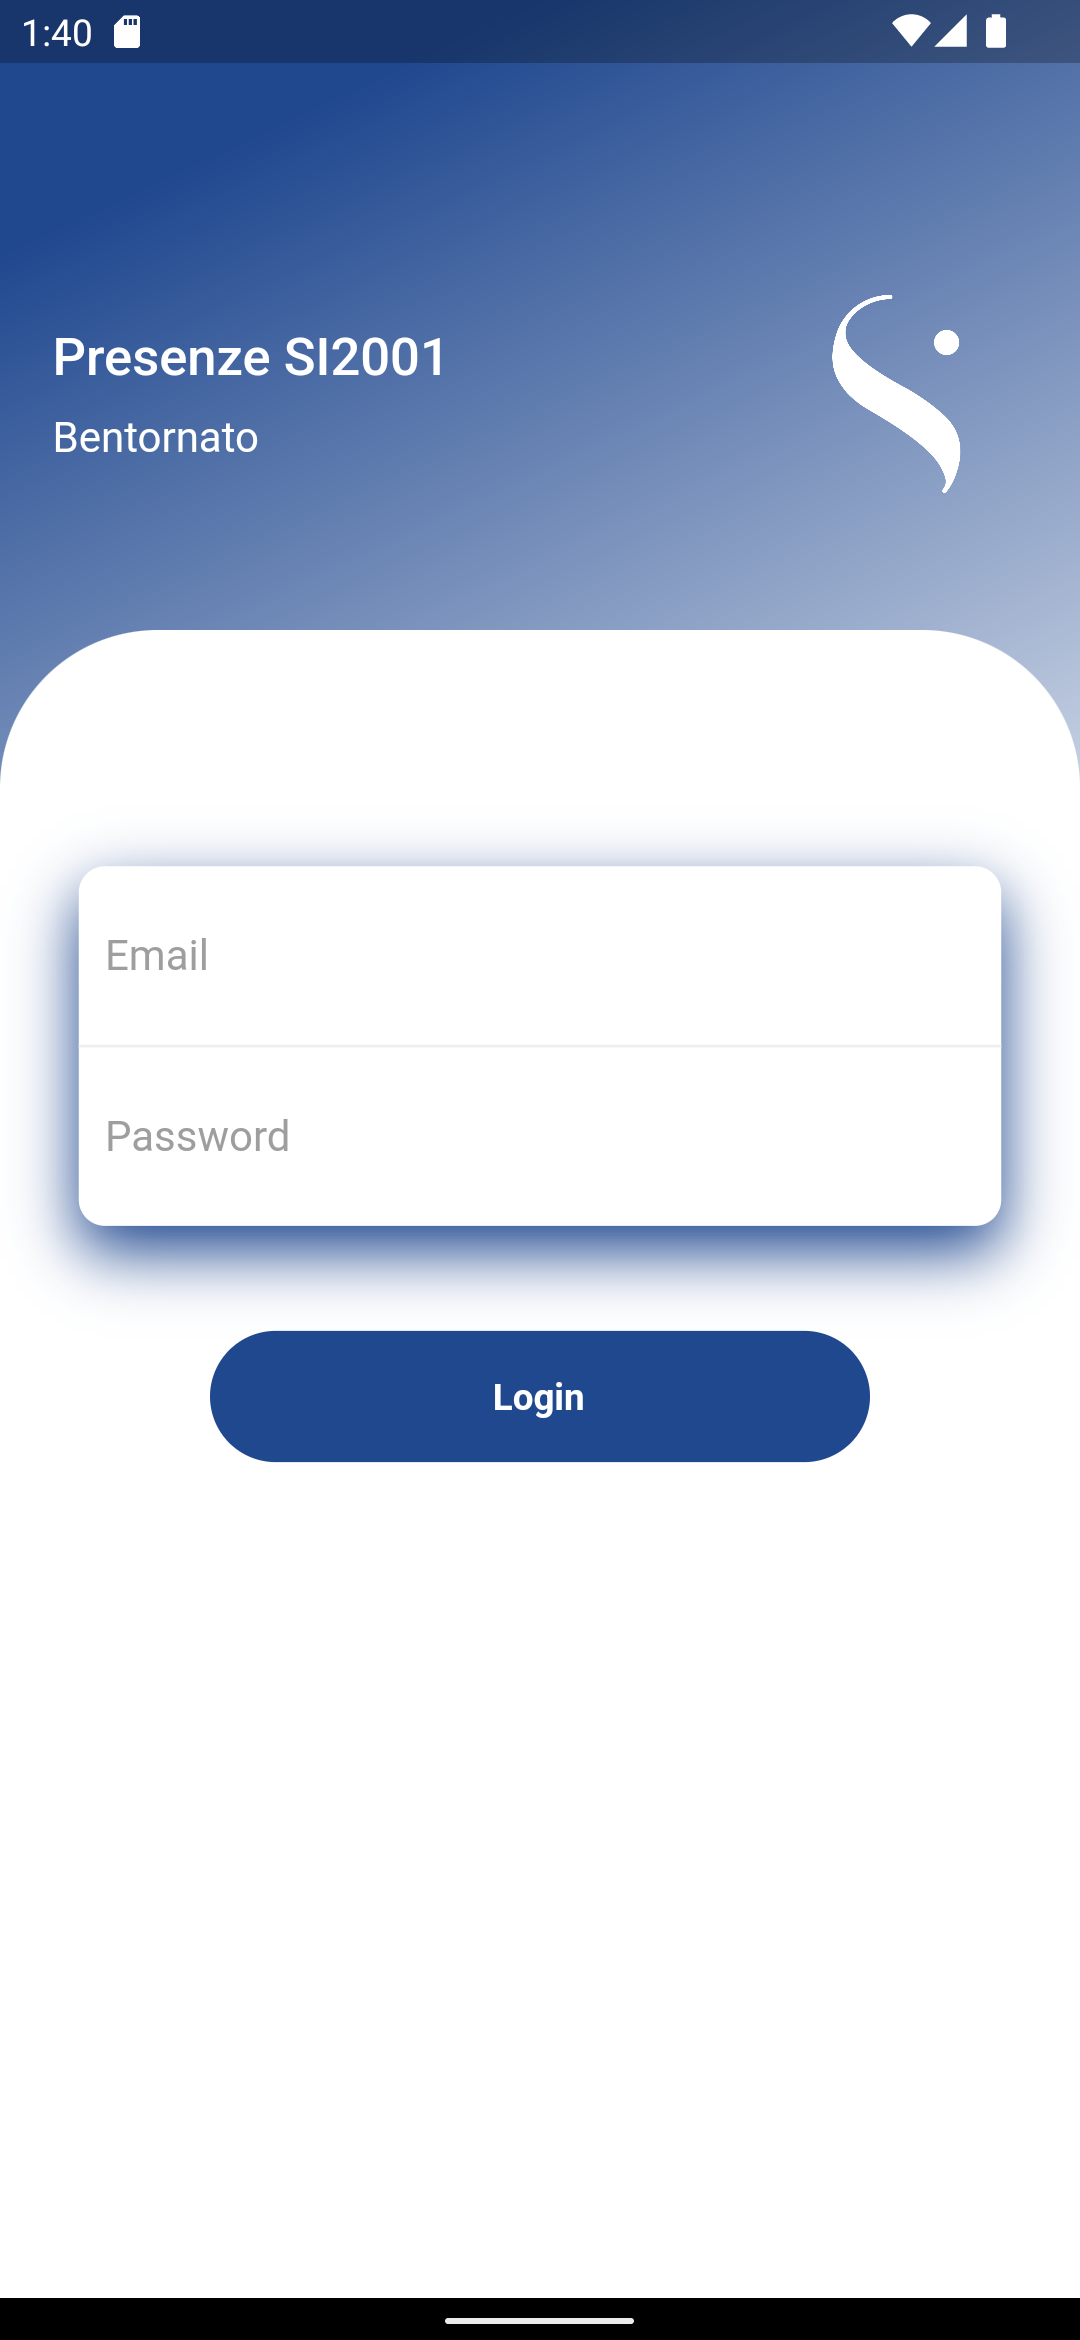
\includegraphics[width=2cm]{../libs/login-page}
				\end{figure}
			\end{column}
			\begin{column}{0.6\textwidth}
				\emph{Alcuni spunti:}
				\begin{itemize}
					\item Aggiungere qualche animazione (Es. Hero, Image Placeholders, Route transitions );
					\item Aggiungere una pagina di dettaglio alla propria sede che ne mostri la posizione dulla mappa
					\item \href{https://pub.dev/packages/flutter_map}{\beamergotobutton{Package mappa suggerito}}
				\end{itemize}
			\end{column}
		\end{columns}
	\end{minipage}
\end{frame}

%% ---------------------------------------------------------------------------

% Reference frames
%\begin{frame}[allowframebreaks]
%    \frametitle{Riferimenti}
%    \printbibliography
%\end{frame}

%% ---------------------------------------------------------------------------
% Final frame
\section{Fine}
\begin{frame}{}
	\huge\emph{Grazie per l'attenzione!}
	\newline
	\vfill
	\hfill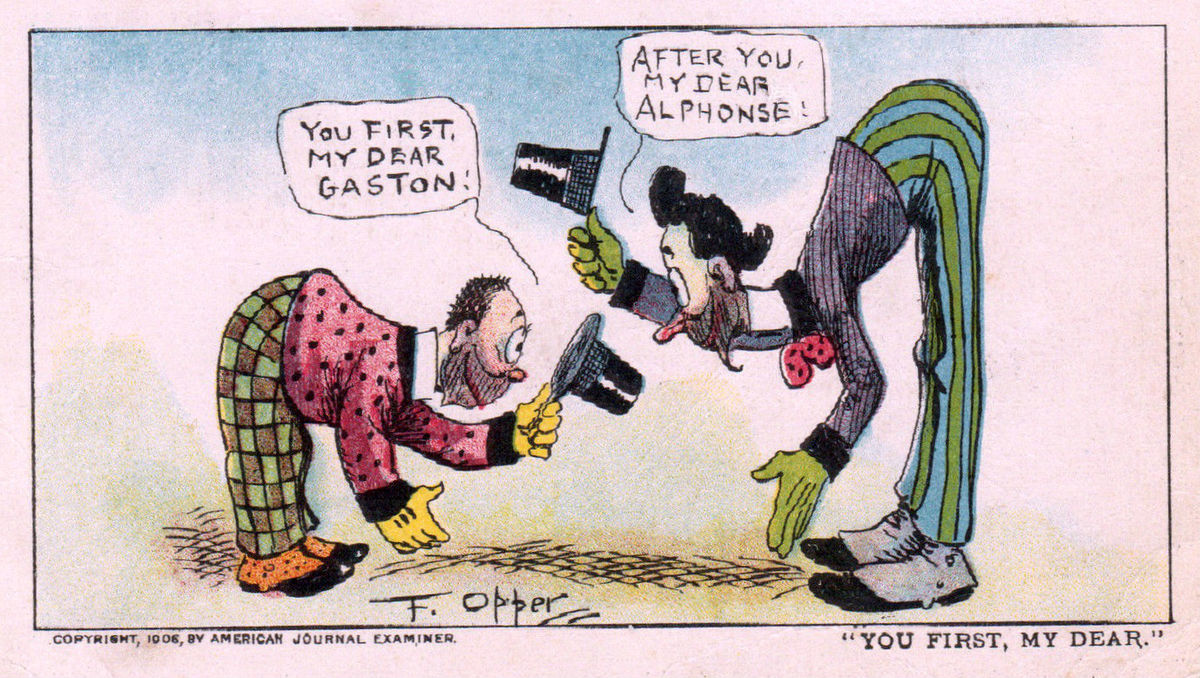
\includegraphics[width=6cm]{../libs/alphonse-gaston-regards}
\end{frame}

\end{document}